\section{Heron of Alexandria: Mechanical Computation in Antiquity}

While modern computation is often traced to the 20th century, the roots of mechanical calculation extend far deeper into history. One of the earliest pioneers was \textbf{Heron of Alexandria} (c.~10--70 AD), whose inventions anticipated key principles of automation, analog computation, and mechanical problem-solving.

\subsection{The Dioptra: Analog Geometry}

Among Heron's most significant contributions was the design of the \textbf{Dioptra}, an advanced surveying instrument used to measure angles, distances, and elevations. Equipped with calibrated scales, rotating parts, and geared mechanisms, the Dioptra allowed users to compute geometric properties mechanically, without the need for complex manual calculations.

In modern terms, the Dioptra functioned as an early \textit{analog computer}: a device that translated proportional geometric relationships into physical measurements through mechanical motion. It mechanized trigonometric processes, enabling accurate land surveying, engineering, and even the planning of aqueducts.

\subsection{Mechanical Automata and Early Programming}

Beyond the Dioptra, Heron explored broader themes of mechanical automation. In his works \textit{Pneumatica} and \textit{Automata}, he described self-operating machines powered by air pressure, steam, water, and mechanical weights. Notable inventions included:

\begin{itemize}
    \item \textbf{The Aeolipile}: A steam-powered rotating sphere---arguably the first known steam engine.
    \item \textbf{Coin-operated Machines}: Devices that dispensed holy water when a coin was inserted, an early form of mechanical vending.
    \item \textbf{Mechanical Theaters}: Programmable automata that enacted miniature plays, using preset sequences of levers, pulleys, and gears.
\end{itemize}

These creations foreshadowed the core ideas of automation and algorithmic control. In essence, Heron's machines demonstrated that mechanical systems could follow conditional sequences---an ancient forerunner of modern programmable computation.

\subsection{Legacy}

Heron's mechanical ingenuity showed that computation could be embodied not only in abstract mathematics but also in physical devices. His work laid a conceptual foundation that, many centuries later, would inspire the design of analog computers, automata, and ultimately the programmable machines of the modern era.

\begin{figure}[H]
    \centering
    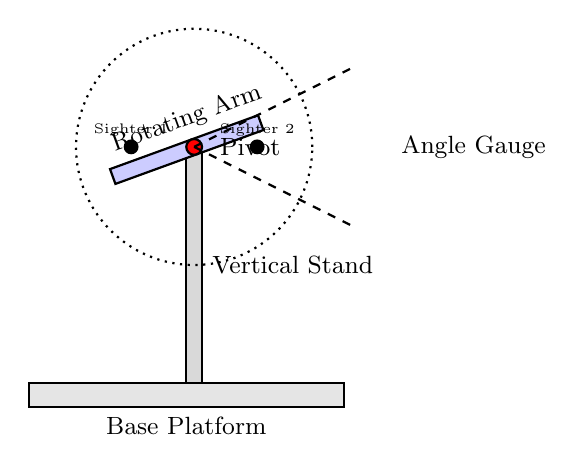
\begin{tikzpicture}[scale=1, thick]
    
    % Base platform
    \draw[fill=gray!20] (-2,0) rectangle (2,-0.3);
    \node[below] at (0,-0.3) {\small Base Platform};
    
    % Vertical stand
    \draw[fill=gray!30] (0,0) rectangle (0.2,3);
    \node[right] at (0.2,1.5) {\small Vertical Stand};
    
    % Rotating horizontal arm
    \draw[fill=blue!20, rotate around={20:(0.1,3)}] (-1,2.9) rectangle (1,3.1);
    \node[above, rotate=20] at (0.1,3.1) {\small Rotating Arm};
    
    % Sighting devices
    \draw[fill=black] (-0.7,3.0) circle (0.08);
    \draw[fill=black] (0.9,3.0) circle (0.08);
    \node[above] at (-0.7,3.0) {\tiny Sighter 1};
    \node[above] at (0.9,3.0) {\tiny Sighter 2};
    
    % Axis of rotation
    \draw[fill=red] (0.1,3) circle (0.1);
    \node[right] at (0.3,3) {\small Pivot};
    
    % Angle gauge
    \draw[dashed] (0.1,3) -- ++(2,1);
    \draw[dashed] (0.1,3) -- ++(2,-1);
    \draw[dotted] (0.1,3) circle (1.5);
    \node[right] at (2.6,3) {\small Angle Gauge};
    
    \end{tikzpicture}
    \caption{Simplified diagram of Heron's Dioptra. The rotating arm, equipped with sighting devices, allowed mechanical measurement of angles and distances.}
    \label{fig:dioptra}
\end{figure}
